\documentclass[10pt,a4paper]{article}
\usepackage[utf8]{inputenc} % para poder usar tildes en archivos UTF-8
\usepackage[spanish, es-tabla]{babel} % para que comandos como \today den el resultado en castellano
\usepackage{a4wide} % márgenes un poco más anchos que lo usual
\usepackage[conEntregas]{caratula}
\usepackage[table]{xcolor}
\usepackage{colortbl}
\usepackage{todonotes}
\usepackage{graphicx}
\usepackage{subcaption}
\usepackage{algorithm}
\usepackage{algorithmic}
\usepackage{dirtree}
\usepackage{cite}
\usepackage{listings}
\usepackage{multirow}
\usepackage{epsfig}

\lstset { %
    language=C++,
    backgroundcolor=\color{green!5}, % set backgroundcolor
    basicstyle=\footnotesize,% basic font setting
}

%definations
\definecolor{Gray}{gray}{0.6}
\definecolor{ligthGray}{gray}{0.9}
\newcommand{\mc}[2]{\multicolumn{#1}{|c|}{#2}}

\begin{document}

\titulo{NetworkDEVS}
\subtitulo{Una herramienta de estudio para medelar redes usando DEVS y PowerDEVS}

\fecha{\today}

\materia{Teoría de las telecomunicaciones}

\integrante{Belloli, Laouen Mayal Louan}{134/11}{laouen.belloli@gmail.com}

\maketitle

\tableofcontents
\newpage

\section{Introducción y Motivación}

El presente trabajo se introduce un modelo DEVS de una red funcionando bajo el protocolo TCP/IP encuadrando lo mejor posible cada uno de sus módulos en su correspondiente capa respecto al modelo OSI presentado en la literatura oficial de la materia de teoría de la telecomunicaciones \cite{peterson2007computer}. El trabajo fue desarrollado en el simulador PowerDEVS y pensado como herramienta de aprendizaje para futuros alumnos de la materia.

El principal aporte de este trabajo consiste en la creación de un framework que permite programar y modificar los protocolos de una red de telecomunicaciones para luego simular su comportamiento y obtener feedback instantáneo de los resultados. Además, usando el simulador PowerDEVS, se consigue brindar una interfaz gráfica intuitiva que mapea de forma directa los dispositivos de la red con los módulos del modelo. Esta interfaz gráfica permite también crear distintos escenarios topológicos sin tener que tocar ni una linea de código. 

Por otro lado, esta interfaz gráfica permite modularizar de forma explicita las distintas capas del modelo y su interacción, mapeando los modelos DEVS de cada capa con su capa correspondiente en la red, permitiendo una interacción más tangible y concreta respecto al modelo en capa. De esta forma, se programa cada protocolo en su capa correspondiente, esto no es menor, ya que si bien, teóricamente, los distintos protocolos están separados en capas y las redes pueden ser pensadas en capas, en la realidad, estas capas no existen de forma explicita y hay un salto entre las teorías de redes y los modelos en capas respecto de sus distintas implementaciones prácticas donde las capas terminan mezclándose en varios aspectos. Este modelo, permite a los alumnos hacer trabajos prácticos donde implementar los protocolos manteniendo explicitas las capas y por ende, acercando la teoría y la práctica de las redes de telecomunicaciones.

Si bien, el modelo realizado es un modelo DEVS (Discrete EVent System Specification), el mismo fue pensado para que no sea necesario más que una breve introducción a DEVS, por lo que mismo personas sin ninguna experiencia en DEVS deberían ser capases de poder utilizar el simulador, el modelo y el framework general propuesto en este trabajo.

\section{Objetivos}

Los objetivos de este trabajo se pueden dividir en varias partes:
\subsection{Desarrollar un framework para modelos de redes}

Como ya fue mencionado en la introducción, uno de los principales objetivos de este trabajo es desarrollar un framework, que permita fácilmente implementar protocolos de red, validarlos y experimentar con ellos mediante Simulación de Eventos Discretos (DES). Ests herramienta permite testear los protocolos implementados de forma sencilla y rápida. Obteniendo una herramienta útil, tanto para el estudio de las redes de telecomunicaciones como para la investigación en el área. 

La creación de un modelo que sirva como framework, tiene por objetivo factorizar y estandarizar las partes comunes a todos los protocolos, estás partes comunes provienen de las propiedades inherentes a los dispositivos físicos en los cuales los protocolos están corriendo, y de los estándares actualmente utilizados que permiten obtener robustez y compatibilidad entre distintas implementaciones que puedan existir en distintas partes de una red. Estas abstracciones encapsuladas en el modelo framework presentado, permiten al modelador, concentrarse plenamente en su protocolo y permite la reutilización y compatibilidad de distintos modelos que pueden luego ser combinados en un único modelo de una red que funcione bajo distintos protocolos, permitiendo así el estudio de la compatibilidad, homogeneidad y efectividad de los protocolos implementados.

\subsection{Modelar una red UDP/IP básica}

Por otro lado, este trabajo pretende implementar un modelo básico de una red UDP/IP que permita cubrir los protocolos mínimos e indispensables para permitir enviar mensajes entre distintos dispositivos. Este modelo no tiene como intensión implementar todas las partes, ni cubrir todos los protocolos de forma completa, por lo que temáticas como la fragmentación de paquetes, congestión de tráfico, manejo de errores, Dinamic Host Configuration Protocol (DHCP) \cite[p.~231]{peterson2007computer}, Routing Information Protocol (RIP)\cite[p.~243]{peterson2007computer} y Spanning tree protocol \cite[p.~194]{peterson2007computer} quedan fuera del alcance de este trabajo, siendo los mismos posibles trabajos futuros.

También se implementó un modelo de switch que utiliza el protocolo de Datagramas \cite{petersonSwitchDatagram} utilizando una forwarding table para enviar los Frames por la interface correspondiente. 

\subsection{Mapeo entre el modelo UDP/IP y el modelo OSI}

En este trabajo, también pretendemos mostrar como se pueden implementar los distintos protocolos del modelo UDP/IP encuadrandolos en un modelo en capas OSI. Para esto, varias decisiones tuvieron que tomarse, siendo tal vez la más difícil, decidir en que capa implementar el protocolo ARP \cite[p.~228]{peterson2007computer}. Para tomar estas decisiones, se tomaron siempre como referencia los textos del libro oficial de la materia \cite{peterson2007computer}. Se intentó también separar lo mejor posible las tareas de cada capa de forma tal que cada una de ellas pueda ignorar lo más posible la existencia de la/las capa/s inferior/es.

\section{Introdución a DEVS}
\section{Introducción a PowerDEVS}
\section{Arquitectura}

\subsubsection{Arquitectura general}
La arquitectura general del modelo propuesto en este trabajo tiene por principal objetivo ofreser un framework donde se pueda facilmente desarrollar protocolos, para esto, se concentra en resolver varios puntos principales:

\begin{itemize}
\item Estandarizar la comunicación entre las capas de forma de conseguir consenso entre los distintos modeladores que usen esta herramienta, y que facilite una comprensión herarquica y organizada del modelo entero para los lectores nuevos.
\item Implementar todas aquellas partes generales a todos los modelos de protocolos de forma que solo sea necesario consentrarse en el protocolo a implementar.
\item intentar minimizar lo más posible la necesidad de tener conocimientos avanzados sobre DEVS a la hora de utilizar la herramienta.
\end{itemize}

La arquitectura consiste en un modelo acoplado ``dispositivo'' de $N$ capas, con $N > 0$ de forma que cada capa $i, i \in [1,..,N]$ se comunica con las capas $i+1$ e $i-1$ utilizando $8$ canales de comunicación distintos:

\begin{itemize}
\item Output port 0: Envio de datos a la capa $i+1$.
\item Output port 1: Envio de controles a la capa $i+1$.
\item Output port 2: Envio de datos a la capa $i-1$.
\item Output port 3: Envio de controles a la capa $i-1$.
\item Input port 0: Recepción de datos de la capa $i+1$.
\item Input port 1: Recepción de controles de la capa $i+1$.
\item Input port 2: Recepción de datos de la capa $i-1$.
\item Input port 3: Recepción de controles de la capa $i-1$.
\end{itemize}

Dado que no siempre sucede que en un dispositivo de la red, exista un solo modulo por capa, y dado que los puertos de salida y entradas estan pensados para comunicarse con un solo modelo en la capa superior/inferior. Es necesario usar modelos demultiplexers que permitan redirigir los mensajes salientes por un puerto al modelo correspondiente de entre todas las posibles opciones. También, se puede usar modelos multiplexers para que los múltiples modelos de la capa superior o inferior envien mensajes al modulo y quede guardado en el campo \textit{interfaz} la ideantidad del modulo de origen del mensaje. \\

Ejemplos de estos son: 
\begin{itemize}
\item Un host que tenga varias aplicaciones enviando datos a travez de distintos sockets y en ese escenario habria más de un módulo en la capa de aplicación (capa siete del modelo OSI) de ese host.
\item  Un router  que tenga más de una interfaz (una por cada sub-red a la cual esté conectado), contando con más de un modulo en la capa de linkeo (capa dos del modelo OSI).
\end{itemize}

Las capas $1$ y $N$ usan la misma arquitectura que el resto de las capas y tienen definidos los mismos puertos. Como que existe solo un medio de comunicación entre dispositivos y tanto datos como controles se envian por ese medio, entonces el modelo acoplado ``dispositivo'' tiene solo un puerto de salida y un puerto de entrada destinado a enviar datos de cualquier tipo, y queda en el modelador decidir que puerto o puertos de salida de la capa $1$ conectar con el puerto de salida del modelo acoplado y que puerto o puertos de entrada de la capa $1$ comunicar con los el puerto de entrada para datos. Por otro lado, el input requerido por la capa $N$ (comunmente el input que indica los pedidos del usuario de enviar o recibir datos) se puede conectar con modelos generadores que pueden estar situados tanto adentro como afuera del modelo acoplado. Lo mismo ocurre con el output generado por la capa $N$ para las capas superiores que no existen; este output puede ser recibido por modelos que lo guardan en archivos y estos modelos también pueden estar situados tanto adentro como afuera del modelo acoplado \\

Distintos dispositivos de la red pueden tener distintas cantidades de capas, por lo cual, la cantidad de capas existente puede variar entre los distintos modelos de cada dispositivo dentro de una misma red. Los hosts por ejemplo, suelen tener hasta la capa siete, mientras que los routers comunes llegan a la capa tres y los switches a la capa dos. \\

La Figura \ref{figure:general architecture} muestra la arquitectura general recien explicada en un modelo de una red con un host y un router, en el mismo se pueden ver: los multiplexers y demultiplexers, modelos con distintas cantidades de capas y las conexiones entre capas utilizando los distintos puertos. \\

\begin{figure}[htbp]
    \centering
    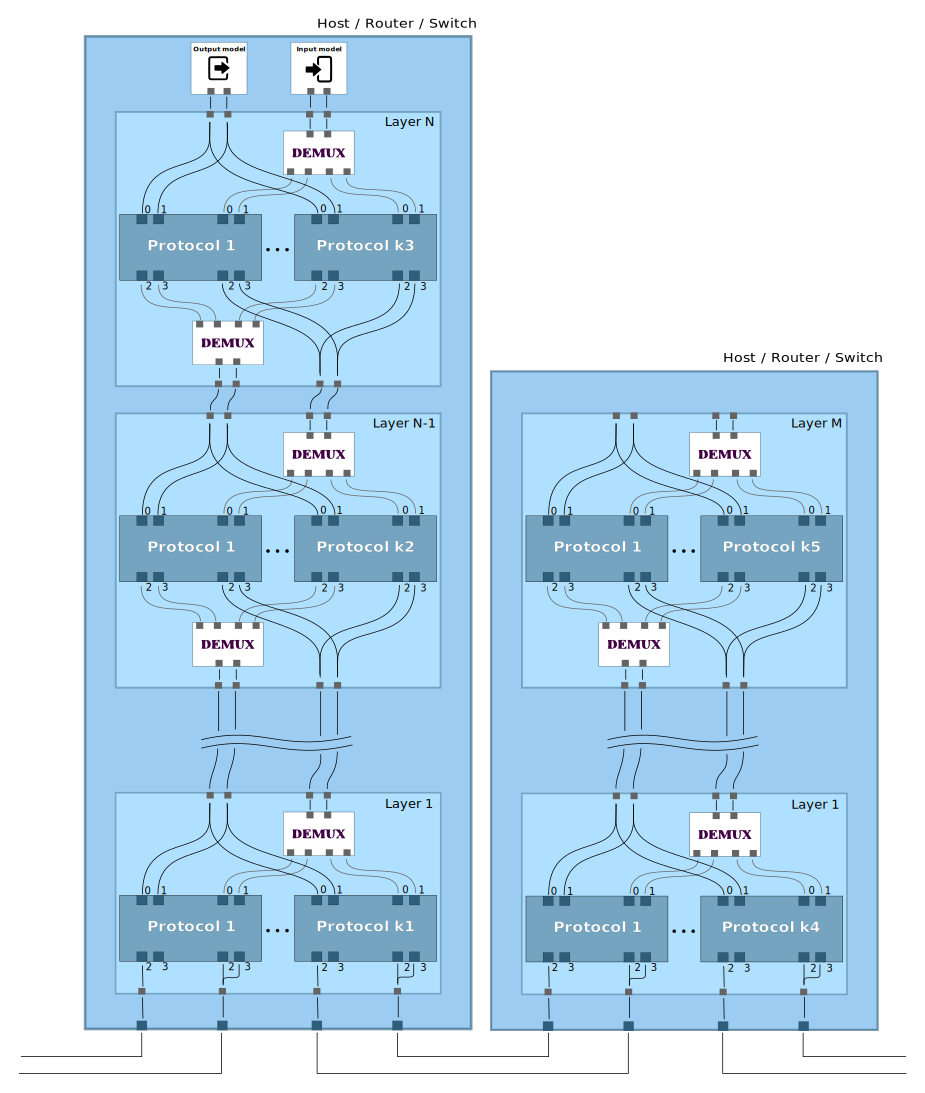
\includegraphics[width = 0.5\textwidth]{img/png/general_architecture.png}
    \caption{Arquitectura de un modelo en NetworkDEVS con dos dispositivos (un host y un reouter de N y M capas correspondientemente).}
    \label{figure:general architecture}
\end{figure}

\newpage

\subsubsection{Arquitectura de las capas}

La arquitectura de las capas está implementado en un modelo template llamado Layer del cual se puede realizar herencia para heredar su estructura. Esta estructura permite abstraer al protocolo de todo el modelo correspondiente al dispositivo, en otras palabras, esta estructura ya modela las propiedades de un dispositivo generico, esto implica manejar el envio y recepción de mensajes a y de otras capas. Para manejar la entrada y salida de mensajes se utilizan colas FIFO; Cada vez que hay un mensajes entrante, el mismo es encolado en la cola de entrada correspondiente y el protocolo los va desencolando y atendiendo de uno o de a muchos dependiendo su implementación, la estructura ya está armada de forma que mientras no halla mensajes por procesar mantiene al modelo pasivado (en estado IDLE) y mientras que hay mensajes por procesar lopea para ir atendiendolos a todos hasta que no halla más mensajes a procesar, momento en el que el modelo se vuelve a pasivar. Por otro lado, cada vez que se quiere enviar un mensaje, el mismo solo debe ser encolado en la cola de mensajes salientes correspondiente dependiendo de si es un mensaje de datos o control a la capa superior o inferior, luego el simulador cuando el protocolo termina el procesamiento actual se encarga de loopear entre las colas de salida para enviar todos los mensajes que hallan sido encolados. La Figura \ref{figure:layer general architecture} muestra la arquitectura deneral de una capa cualquiera y la Figura \ref{figure:processing flow} muestra el flujo de procesamiento generado por el modelo template cuando es extendido agregandole un protocolo.

\begin{figure}[htbp]
    \centering
    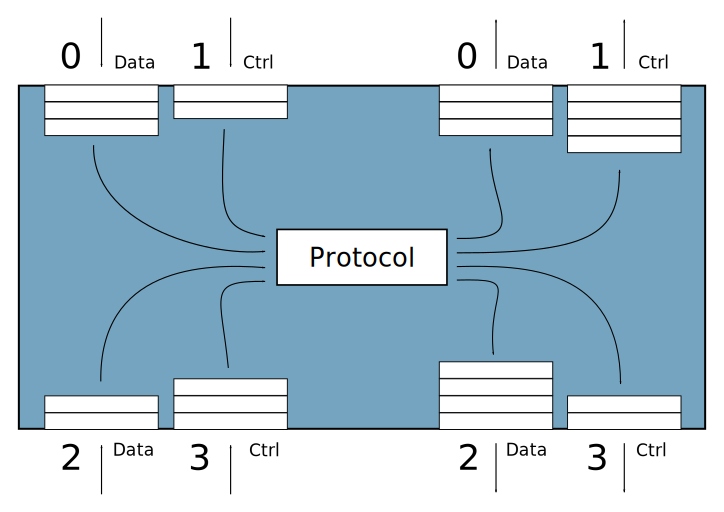
\includegraphics[width = 0.4\textwidth]{img/png/layer_architecture.png}
    \caption{Arquitectura de una capa en NetworkDEVS.}
    \label{figure:layer general architecture}
\end{figure}

\begin{figure}[htbp]
    \centering
    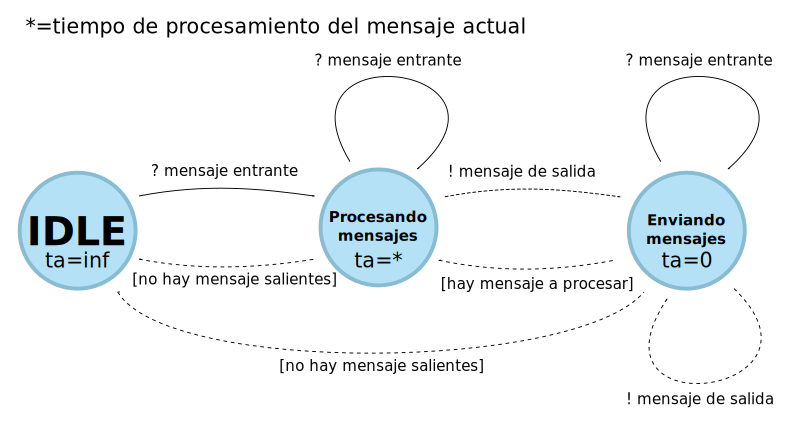
\includegraphics[width = 0.6\textwidth]{img/png/processing_flow.png}
    \caption{Flujo de procesamiento de una capa que extiende al modelo template Layer.}
    \label{figure:processing flow}
\end{figure}

\section{Como usar el template}

Todo el modelo está implementado en C++ y la forma de usar el template es mediante la implementación de herencias. Para poder comprender como utilizarlo, primero introduciremos la estructura de archivos del framework. \\

\dirtree{%
.1 NetworkDEVS.
.2 libs.
.3 logger.h.
.3 message\_queue.h.
.3 parser.h.
.2 structures.
.3 bastract\_types.h.
.3 app.h.
.3 ip.h.
.3 ipv4.h
.3 link.h.
.3 mac.h.
.3 socket.h.
.3 sw.h.
.3 swp.h.
.3 udp.h.
.2 templates. 
.3 layer.h.
.3 demultiplexer.h.
.3 multiplexer.h.
.2 top.pdm.
.2 top.pds.
.2 top.stm.
}

\medskip

La carpeta \textit{structures} es la que contiene las definiciones de todos los tipos de datos que vienen por defecto con el framework, algunos de ellos fueron implementados exclusivamente para el modelo presentado en este trabajo, pero todos pueden ser utilizados y están incluidos por el modelo template Layer que introduciremos a continuación. Los tipos de datos están implementados usando structs y casi todos heredan de dos tipos abstractos definidos en \textit{abstract\_types.h} que sirven como organizadores, de esta forma quedan están separados entre los que son Data y los que son Headers. Cada tipo de dato definido cuenta con documentación en el código en formato Doxigen y la misma fue exportada y se encuentra disponible en el apendice de este documento. \\

Todos los tipos de datos estan implementados en namespaces que sirven como organizadores, para cada capa existente debe existir un namespace y los tipos de datos inherentes a esa capa (por más que otras capas lo usen) tienen que estar definidos dentro del namespace. Si se implementan nuevas capas, se deben crear sus correcpondientes namespaces a menos que no halla tipos de datos correspondientes a la capa. De está forma se evitan las ambiguedades, que son muy recurrentes en el ambito de las redes.

\subsection{Como heredar el modelo layer}

El modelo Layer es el modelo template que contiene toda la implementación correspondiente a la arquitectura general de una capa. El mismo es un modelo que cuenta con 4 tipos de datos templates a instanciar y 4 tipos de datos template con instanciación por defecto si no se explicitaran otros tipos para ellos. Estos tipos a instanciar son los tipos de los mensajes que envian y reciben los puertos y los tipos con los cuales se definen las colas. Por defecto se asume que los puertos de entrada y salida del mismo tipo de mensajes (Datos o Control) para y desde la misma capa, tienen el mismo tipo. Es por esto que hay solo 4 tipos template que deben ser instanciados obligatoriamente, mientras que los restantes cuatro se mapean por defecto con los primeros 4 para conseguir sus tipos.\\

El modelo Layer tiene la siguiente forma:
\begin{lstlisting}
template <typename DH, CH, DL, CL, DH2 = DH, CH2 = CH, DL2 = DL, CL2 = CL>
class Layer: public Simulator { 

protected:
  // Logger
  Logger logger;

  // Input queues
  std::queue<DH> higher_layer_data_in; // Input Port 0
  std::queue<DL> lower_layer_data_in;  // Input Port 1
  std::queue<CH> higher_layer_ctrl_in; // Input Port 2 
  std::queue<CL> lower_layer_ctrl_in;  // Input Port 3
  
  // Output queues
  msg::queue<DH2> higher_layer_data_out; // Output Port 0 
  msg::queue<DL2> lower_layer_data_out;  // Output Port 1
  msg::queue<CH2> higher_layer_ctrl_out; // Output Port 2
  msg::queue<CL2> lower_layer_ctrl_out;  // Output Port 3

  Event output;

  double next_internal;
  double last_transition;
  double infinity = std::numeric_limits<double>::max();
  bool queuedMsgs() const { ... }

public:

  Layer(const char *n): Simulator(n) {};
  double ta(double t);  
  Event lambda(double);
  void dint(double t) { .... }
  void dext(Event x, double t) { .... }
  
  virtual void dinternal(double t) {}
  virtual void dexternal(double t) {}
};
\end{lstlisting}

PowerDEVS tiene un par de exigencias a la hora de declarar un nuevo modelo, por este motivo, a continuación se muestra un ejemplo de herencia que puede ser usado de base para implementar nuevos modelos de capas. \\

\newpage

\textbf{protocol\_name.h}
\begin{lstlisting}
//CPP:path_to_cpp_files/protocol_name.cpp
#include "layer.h"

class layer_name: public Layer<T1, T2, T3, T4> { 

protected:
	
  // variables privadas del modelo
  // metodos privados del modelo

public:
  protocol_name(const char *n): Layer(n) {};
  void init(double, ...);
  void exit();

  virtual void dinternal(double);
  virtual void dexternal(double);
  
  // variables publicas del modelo
  // metodos publicos del modelo
};
\end{lstlisting}

\textbf{Exigencias}
\begin{itemize}
\item La primer linea es requerida por el compilador de PowerDEVS y tiene que tener correctamente seteado la dirección al archivo \textit{.cpp} donde estén implementados todos los métodos del modelo.
\item El constructor de la clase debe estar declarado como se muestra en el ejemplo y la función init es la utilizada por el simulador para inicializar el modelo. Esta función debe ser declarada como se muestra con los \ldots, el simulador llama a esta función pasandole como primer parametró \textit{double} la cantidad de párametros a leer y luego el resto de los parámetros definidos para el modelo en la IDE PowerDEVS, los mismos se recuperan utilizando la librería \textit{va\_start} y \textit{va\_arg}.
\item El método exit también debe ser declarado y el mismo es llamado por el simulador al finalizar la simulación. Todos los destructores correspondientes deben ser llamados en esta función de forma de liberar correctamente la memoria.
\item El nombre de la clase debe estar escrito todo con minúsculas.
\end{itemize}

Como se puede observar existen las funciones \textit{dint} y \textit{dext} que son las funciones exigidas por el simulador para ejecutar correctamente las transiciones interna y externa correspondientes al formalismo DEVS, el modelo Layer ejecuta en esas funciones todo el código relativo a la arquitectura presentada y llama a los métodos virtuales \textit{internal} y \textit{dexternal} que son sobre escritos por el modelador para ejecutar el protocolo implementado. De esta forma se consigue abstraer lo más posible al modelador del formalismo, convirtiendo esta herramienta en una herramienta viable para el uso dentro del ambito de estudio. \\

Por otro lado, la variable \textit{next\_internal} definida en en el template Layer es inicializada en cero cada vez que se llama a la implementación del protocolo, y es utilizada por el modelo para agendar la próxima transición interna, de esta forma si el protocolo no asigna ningún valor a esta variable, el simulador genera una transición interna instantanea. El desarrollador del protocolo tiene que asignar en esta esta variable un modelo del tiempo de computo del protocolo para de esta forma modelar los tiempos reales de runtime. Esta variable es de tipo double y la representación del tiempo mediante doubles queda en manos del modelador y debe ser consensuada con el resto de los modeladores de los demás protocolos para poder unirlos en un solo modelo, un consenso común es asumir que un double representa un segundo y utilizarlo de forma similar a los timestamps. \\

\subsection{Como enviar y recibir mensajes entre las capas}

Todos los mensajes que llegan al modelo de una capa son recibidas por uno de los cuatro siguientes puertos dependiendo de donde provenga el mensaje:
\begin{itemize}
\item std::queue$<DH>$ higher\_layer\_data\_in:  Input Port 0
\item std::queue$<DL>$ lower\_layer\_data\_in:   Input Port 1
\item std::queue$<CH>$ higher\_layer\_ctrl\_in:  Input Port 2 
\item std::queue$<CL>$ lower\_layer\_ctrl\_in:   Input Port 3
\end{itemize}

La Figura \ref{figure:layer general architecture} Muestra de que capa proviene y para que tipo de datos está pensado cada uno de estos puertos. \\

Como ya fue mencionado y como se puede observar en la definición de las colas, los tipos template instanciados son los tipos de los mensajes recibidos desde las capas superior e inferior. Es importante que los mensajes recibidos sean efectivamente de este tipo, porque el simulador PowerDEVS envia mensajes como \textbf{void *} y los mismos son casteados a su tipo correspondientes una vez recibidos por el modelo receptor, por lo que si los tipos no corresponden se generará un excepción en tiempo de ejecución. \\

Para procesar los mensajes, dentro del método \textit{internal}, los mismos deben ser desencolados, es importante que se desencolen, ya que en caso contrario el mismo seguirá estando en la cola y el modelo volverá a producir una transición interna y llamar de nuevo al método \textit{internal} procesando dos o más veces el mismo mensaje. Reprocesar un mensaje multiple veces probablemente esté mal, pero tal vez es lo deseado por el protocolo, pero hay que tener en cuenta que una de las pocas exigencias del formalizmo DEVS es que no ocurran infinitos eventos en un mismo momento del tiempo virtual, y como el modelo sigué generando transiciones internas mientras haya mensajes por procesar, si los mensajes no son nunca desencolados y la variable \textit{next\_internal} se mantiene en cero, se generan infinitas transiciones internas y eso produciría un modelo DEVS ilegítimo que cuelga al simulador. \\

Para enviar mensajes las colas a utilizar son las siguientes:
\begin{itemize}
\item msg::queue$<DH2>$ higher\_layer\_data\_out: Output Port 0 
\item msg::queue$<DL2>$ lower\_layer\_data\_out:  Output Port 1
\item msg::queue$<CH2>$ higher\_layer\_ctrl\_out: Output Port 2
\item msg::queue$<CL2>$ lower\_layer\_ctrl\_out:  Output Port 3
\end{itemize}

Como se puede observar, los nombres de los tipos a instanciar son iguales a los de las colas de entrada con un $2$ al final, esto es porque los mismos por defecto se instancian usando los tipos de las colas de entrada a menos que en la declaración de la herencia se especifique lo contrario, esto es así ya y se considera buena práctica que el tipo de datos que intercambian dos capas por un canal de comunicación sea siempre el mismo en ambas direcciónes, facilitando la reutilización y comprensión de los modelos por parte de otras personas. \\

Para encolar un mensaje en la cola de de salida correspondiente se debe utilizar el método \textit{msg::queue::push(MSG mensaje)}. De la misma forma que el modelo Layer se encarga de encolar los mensajes en la cola de entrada correspondiente dependiendo el puerto por donde llegó el mensaje, el mismo se encarga de desencolar y enviar los mensajes encolados en las colas de salidas por el puerto correspondiente a cada cola y desencolar el mismo. \\

El tipo de datos msg::multiplexed$<typename MSG>$ sirve para enviar mensajes que van a ser demultiplexados por un modelo demultiplexer$<typename MSG>$. El mismo cuenta con los campos \textit{message} e \textit{interface} que son utilizados para asignar el mensaje y el identificador del destinatario. Luego solo resta utilizar un modelo demultiplexer, setear correctamente sus parámetros en la IDE de PowerDEVS, y conectar correctamente sus puertos de entrada y salida con el modelo de origen y los modelos de destino. La Figura \ref{figure: demultiplexer} muestra como es el mapeo de los puertos de un demultiplexer conectado a \textit{k} modulos\footnote{En el modelo implementado en este trabajo hey ejemplos de como utilizar el modelo demultiplexer con el tipo de dato msg::multiplexed}\footnote{Un demultiplexer con relación $1$ a $k$ numera los modulos de salida de $0$ a $k-1$}. \\

\begin{figure}[htbp]
    \centering
    
\includegraphics[width = 0.6\textwidth]{img/png/demultiplexer.png}
    \caption{Puertos de entrada y salida de un demultiplexer, mapeo del campo interfaz del mensaje multiplexado con el puerto de salida correspondiente.}
    \label{figure: demultiplexer}
\end{figure}

Para no tener que usar un demultiplexer para los mensajes de datos y otro demultiplexer para los mensajes de controles, el modelo demultiplexer cuenta con dos puertos de entrada (datos y controles) y envia los mensajes por los puertos pares si son datos y por puertos impares si son controles; De esta forma, un mensaje de control que llega con interface $i$ es enviado por el puerto $2*i+1$ y un mensaje de datos que llega con interface $i$ es enviado por el puerto $2*i$. \\

El campo \textit{interface} le indica al demultiplexer por que puerto enviar el mensaje, por lo que es importante conectar correctamente los puertos de salida del demultiplexer correctamente con los destinatarios, la entrada de datos del modelo $i$ de destino debe estar conectado al puerto de salida $2*i$ del demultiplexer y la entrada de controles del modelo $i$ debe estar conectado al puerto $2*i+1$ del demultiplexer. \\

\subsection{Como implementar el protocolo de una capa (internal/external functions)}

El template cuenta con dos métodos virtuales que están definidos e implementados como funciones vacias (sin comportamiento), estos métodos son los que deben ser sobre escritos para implementar el protocolo. Siempre que haya mensajes por procesar en las colas de entradas, el modelo llama al método \textit{internal} en el cual se deben procesar dichos mensajes, el modelo Layer mira las colas de salidas para ver si hay mensajes a enviar y los envia, si al finalizar este proceso sigue habiendo mensajes por procesar en la cola de entrada se volverá a llamar a esta función respetando el formalismo DEVS de forma de seguir procesando mensajes. Este ciclo se repite indefinidamente hasta que no haya mas mensajes por procesar, momento en el cual el modelo se pasiva a la espera de nuevos eventos externos. \\

El método virtual \textit{dexternal} existe por si se desea implementar código que se ejecute cada vez que ocurre un evento externo para modificar el estado de las variables internas del protocolo o por algún otro motivo. Esto no es recomendado para desarrolladores no familiarizados con el formalismo DEVS o PowerDEVS. \\

\section{Como agregar una capa}

Como ya vimos en la sección ``introducción a DEVS'', hay dos tipos de modelos: los modelos atómicos y los modelos acoplados. Para implementar un modelo de capa, primero es necesario heredar del template Layer para obtener el modelo atomico capa como fue descripto en la sección anterior y luego el mismo debe ser insertado mediante la IDE PowerDEVS dentro del modelo acoplado general. \\

Como se muestra en la arquitectura general, las capas deben ser insertadas dentro de los modelos acoplados de dispositivos (hosts, switches, routers, etc), por lo que antes de agregar la capa al modelo hay que abrir el modelo acoplado dispositivo en caso de existir, o crear el modelo acoplado dispositivo en caso de todavía no existir.

\begin{itemize}
\item \textbf{Abrir un modelo acoplado en PowerDEVS:} Seleccionar con el mouse el modelo acoplado a abrir y desplegar el menú de opciones del mismo dando click derecho sobre el icono, luego elegir la opción ``open model''.
\item \textbf{Crear un modelo acomplado en PowerDEVS: } Abrir la pestaña ``Basic Elements'' del sector ``library'' de la IDE y arrastrar el icono ``Coupled'' desde el menú hasta el sector donde esta el dibujo del modelo.
\end{itemize}

La figura \ref{figure: PowerDEVS IDE} muestra la IDE PowerDEVS e indica como crear un modelo acoplado dentro de la misma. \\

\begin{figure}[htbp]
    \centering
    \includegraphics[width = 0.6\textwidth]{img/png/powerDEVS_coupled.png}
    \caption{Screenshot de la IDE PowerDEVS con la pestaña ``Basic Elements'' abierta resaltando el ícono de coupled model.}
    \label{figure: PowerDEVS IDE}
\end{figure}

Para insertar un nuevo modelo de capa dentro de un modelo acoplado de dispositivo en PowerDEVS hay que seguir los siguientes pasos:

\begin{enumerate}
\item Crear el modelo acoplado de dispositivo (en caso de ser necesario) y abrirlo.
\item Crear un nuevo modelo atómico de capa:
\begin{enumerate}
\item De la solapa ``Basic Elements'' arrastrar al escenario el icono ``atomic''.
\item Click derecho sobre el icono del nuevo modelo atomico en el escenario.
\item Elegir la opción  ``edit''.
\item Ir a la pestaña ``code'', navegar por los modelos hasta encontrar el archivo \textit{.h} del modelo capa creado y seleccionarlo.
\item Ir a la pestaña ``parameters'' y agregar todos los parámetros requeridos por el modelo, o sea aquellos que el simulador le va a pasar al método ``init'' del modelo para inicializarlo y que serán leidos usando \textit{va\_arg} \footnote{Estos parámetros dependen de la implementación particular del protocolo.}.
\item Ir a la pestaña ``properties'' y realizar las siguientes tareas: Escribir el nombre deseado para el nuevo modelo, setear cuatro puertos de entrada y cuatro puertos de salida y elegir el icono a mostrar en el modelo (Elegir un ícono no es obligatorio)
\end{enumerate}
\item Conectar las salidas de los modelos superiores e inferiores con las entradas del nuevo modelo según lo explicado anteriormente en la sección \textit{Como enviar y recibir mensajes entre las capas}.
\item Conectar las salidas del nuevo modelo a las entradas correspondientes de los modelos de las capas superiores e inferiores según lo explicado anteriormente en la sección \textit{Como enviar y recibir mensajes entre las capas}.
\end{enumerate}

\todo[inline]{Colocar figuras ilustrativas de los pasos anteriores.}

\section{Input/output del modelo}

\subsection{Input}
Existen dos módulos responsables de leer el/los inputs del modelo, estos son: El modelo atómico template \textit{input\_stream} y la clase \textit{Parser}. La idea de separar el input en dos módulos es la de atacar dos problematicas distintas pero similares:

\begin{itemize}
\item Contar con un parser que sepa leer archivos utilizados para inicializar modelos que requieren parámetros muy grandes \footnote{como por ejemplo las inicializaciones de las diferentes tablas utilizadas por el modelo (routing/forwarding tables)}.
\item Contar con un modelo generador que utilice el parser y se encargue de ir insertando los estimulos externos al modelo en el tiempo virtual correspondiente.\\
\end{itemize}

\newpage

\subsection{La clase Parser}
Esta clase está diseñada como template y sirve para leer las lineas de un archivo y parsearlas con el fin de devolverlas en la estructura de datos correspondiente según la instanciación realizada. El \textit{typename INPUT} indica el tipo del input a parsear y el mismo debe implementar el operador std::istream \textsf{operator}$>>$(\textsf{std::istream}\& is, \textsf{IPv4}\& ip). Es importante que este operador este implementado de forma que lea todos los atributos necesarios sin saltos de linea ya que el parser lee un input por linea.\\

El constructor de la clase Parser recibe como parámetro un valor boleano que indica si el input a leer viene asociado con un tiempo (un valor \textit{double}). En caso de que este parámetro sea \textit{true}, las lineas del archivo deben comenzar con un valor \textit{double} que será devuelto por el parser de forma separada al input y que representa el tiempo en que debe ser insertado el input en la simulación, luego debe haber un espacio y el resto de la sintaxis requerida por el operador $>>$ del tipo de datos a parsear. Si bién el Parser tiene la opción para parsear el input junto con un tiempo asociado, el mismo no hace más que devolverlo en una tupla (tiempo, mensaje).\\

La clase Parser puede ser utilizada de forma independiente al modelo que lee input siempre que sea necesario leer y parsear las lineas de un archivo. La interfaz y documentación técnica del Parser está en formato Doxigen y exportado en el apendice de este documento.

\subsection{El modelo input stream}

El modelo input stream es un modelo handler que se encarga de manejar el parser de forma de ir leyendo el input e ir insertándolo en el momento correcto de la simulación. Para esto, el modelo está implementado como template de forma de poder funcionar con distintos tipos de inputs, el parámetro template es el mismo que se utiliza para iniciar el parser. \\

Para utilizar este modelo, hay que crear una clase input\_stream\_$<$tipo del input$>$ que herede de input\_stream \footnote{El archivo header siempre tiene que ser de tipo \textit{.h} y la implementación debe estar en un archivo \textit{.cpp}} instanciando el parámetro template. Dado que el simulador PowerDEVS requiere que los modelos tengan un archivo \textit{.cpp} el mismo debe existir y puede simplemente estar vacio. \todo[]{Agregar en todos los lugares donde se introducen modelos, la tabla con los parametros a instanciar en la IDE PowerDEVS y que tipo de datos es cada parámetro.} \\

Una vez creada la herencia, el modelo atómico está listo para ser utilizado, el mismo no tiene ningún puerto de entrada y un solo puerto de salida por donde salen los inputs generados, este puerto de salida es el que debe ser conectado al modelo que precisa del input.

\section{Logger}

La clase Logger sirve para ir creando logs de la simulación. Esta clase separa los logs en cuatro tipos:

\begin{itemize}
\item \textbf{LOG:} Logs que sirven para documentar eventos no relevantes de la simulación.
\item \textbf{INFO:} Logs utilizados para documentar eventos relevantes de la simulación.
\item \textbf{DEBUG:} Logs utilizados para documentar eventos que sirven de ayuda para tareas de debug pero que no tiene ningún otro interés.
\item \textbf{ERROR:} Logs utilizados para documentar errores producidos en tiempo de ejecución.
\end{itemize}

Para habilitar y deshabilitar los distintos tipos de logs a guardar en una simulación solo hay que comentar y descomentar las lineas $4,5,6$ y $7$ del archivo \textit{logger.h}, de esta forma en el código se logean todos los eventos correspondientes a estas cuatro categorías y luego antes de cada simulación se decide que mensajes mostrar y cuales no. \\

Lineas a descomentar y comentar para habilitar y deshabilitar los distintos tipos de logs correspondientemente:
\begin{lstlisting}
#define show_log
#define show_info
#define show_debug
#define show_error
\end{lstlisting}

Para utilizar esta clase, cada modulo tiene que crear una variable de tipo \textit{Logger} e inicializarla pasandole como parámetro un \textit{string} con el nombre del módulo o modelo del cual el logger va a loggear eventos y luego utilizarlo siguiendo su interfaz. La inicialización de la variable puede ser en su constructor o mediante el método \textit{Logger::setModuleName(std::string other\_module\_name)}. La documentación de la interfaz está en formato Doxigen y adjunto en el apendice de este documento. \\

\section{Caso de estudio}
	Además de implementar un framework para el estudio de las redes, en este trabajo se introduce un modelo sencillo del protocolo UDP/IP, el mismo cuenta con los protocol necesarios para que la red funcione de forma que los mensajes van pasando a travez de las distintas capas para llegar a ser enviados de un dispositivo a otro. La Figura \ref{figure: protocolos} muestra un diagrama de los protocolos implementados. \\

\begin{figure}[!htb]
    \centering
    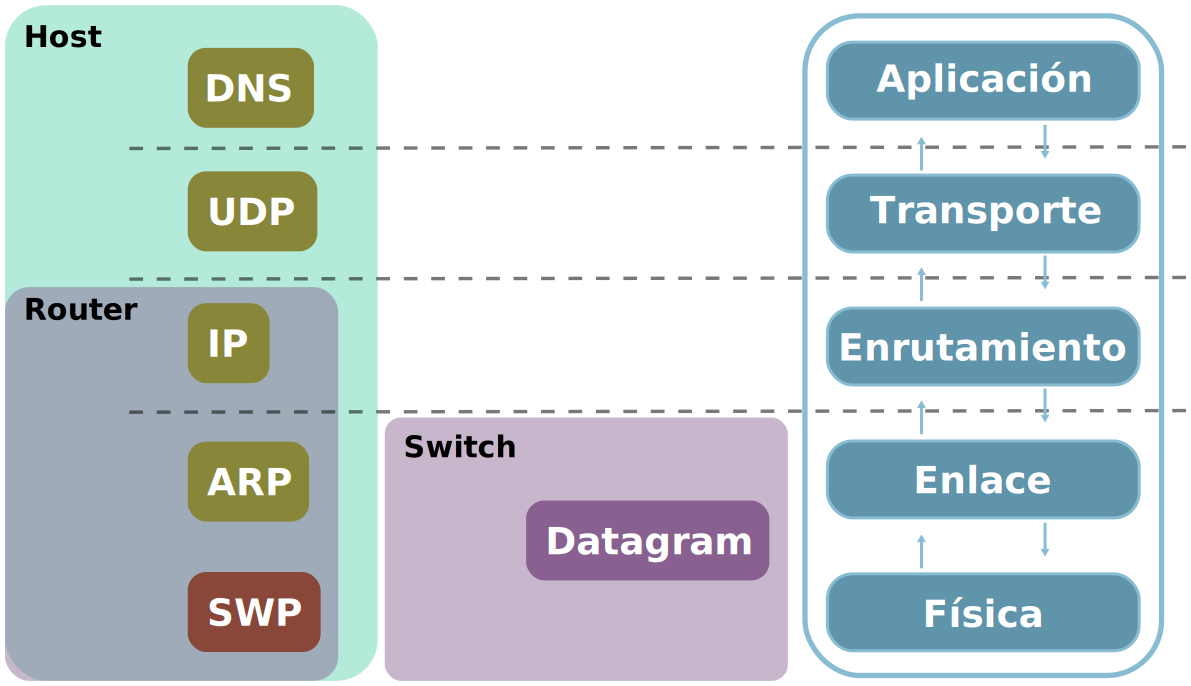
\includegraphics[width = 0.8\textwidth]{img/png/protocols.png}
    \caption{Protocolos implementados separados por capas y dispositivos que los utilizan.}
    \label{figure: protocolos}
\end{figure}
	
\subsection{HTTP}
\subsection{UDP}

\subsection{Estructuras de datos correspondiente a UDP}

El protocolo UDP implementado cuenta con los siguientes tipos de datos, los cuales cuentan con documentación en formato Doxigen y que se encuentra adjunto en el apéndice de este documento:
\begin{itemize}
\item udp::Segment: Representa un segmento de datos para ser enviado por la red, el mismo cuenta con pseudoheader, header y payload como se muestra en la Figura \ref{figure: udp segment}.
\item udp::Control: Es la estructura de datos utilizada para la comunicación con la capa de aplicación, en la misma se especifica que comando envia la aplicacion a la capa UDP. Toda la información a enviar llega al protocolo UDP a travez de esta estructura.
\end{itemize}

\begin{figure}[!htb]
    \centering
    \includegraphics[width = 0.6\textwidth]{img/png/UDP-Segment.png}
    \caption{Estructura del tipo de datos udp::Segment}
    \label{figure: udp segment}
\end{figure} \todo[]{Redibujar para que esté en español}

\subsection{Comportamiento del protocolo}

El protocolo UDP no cuenta con ningún sistema de detección de fallas en la entrega de los mensajes ya que el mismo está pensado para funcionar de forma que optimise la velocidad de entrega, para esto se basa en un mecanismo de mejor esfuerzo. Esto lo convierte en un buen protocolo cuando la eficiencia es un atributo clave. Por otro lado, dado que no controla que los mensajes lleguén o no a su destino, es necesario contar con otro mecanismo que detecte mensajes faltantes (aquellos que no llegaron a destino) o de lo contrario, debe permitirse la perdida de los mismos. Si bien no se realiza ningún esfuerzo por detectar si el mensaje llega o no a destino, UDP implementa checksum para detectar errores en la codificacion del header del segmento, esto es implementado con la finalidad de no entregar mensajes a destinatarios incorrectos. Cuando un error es detectado en el header, el segment es directamente descartado\footnote{No se comprueba que el payload contenga errores en su codificación, por lo que el dato en si, podria llegar a destino con errores y nunca serían detectados por UDP.}.\\

UDP funciona con sockets, los sockets son una conbinación de IP y puerto que permiten enviar y entregar los mensajes a la aplicación correspondiente  dentro del host de destino. De esta forma, para que un mensaje sea correctamente entregado, el host destino tiene que tener una aplicación que esté escuchando por el puerto al cual fue enviado el mensaje, si este no es el caso, el mensaje es simplemente descartado. Los sockets también cumplen el roll de evitar colisiones entre las aplicaciones ya que las mismas no pueden conectarse a un puerto mediante un socket si el puerto ya está siendo utilizado por otra aplicación, ya sea para enviar o recibir mensajes. La Figura \ref{figure: UPD flow} muestra la máquina de estados del protocolo UDP. \\

\todo[inline]{Colocar figura de la máquina de estados de UDP}
 
En el modelo implementado, los mensajes de Control contienen un campo \textit{request} que indica que operación se desea efecectuar (connect, bind, read, etc) también es necesario enviar el IP y puerto del socket y el id de la aplicación, esta información es siempre requerida, ya sea para crear un nuevo socket atado a la aplicación del id o para corroborar que el socket existe y que corresponde a la aplicación que envia el mensaje de control. Dependiendo de la operación, es preciso completar correctamente los campos restantes. A continuación se explica cada operación y que campos requiere cada una: \\

\begin{itemize}
\item \textbf{CONNECT}: \textit{remote\_ip}, \textit{remote\_port}. De está forma UDP sabe que cada vez que esta aplicación envie o reciba un paquete, el mismo será para o desde el socket con IP \textit{remote\_ip} y puerto \textit{remote\_port}. Esta operación falla si el socket ya existe.
\item \textbf{BIND:} Esto permite a la aplicación enviar paquetes a distintos destinos, especificando siempre el socket del destino mediante los comandos WRITE\_TO y SEND\_TO y recibir mensajes de distintos orígenes mediante los comandos READ\_FROM, RECV\_FROM, REC o READ. Esta aplicación falla si el soquet ya existe.
\item \textbf{READ\_FROM / RECV\_FROM:} \textit{remote\_ip}, \textit{remote\_port}, estos campos son utilizados para saber que mensajes entrantes deben que ser aceptados y cuales no. Cuando este comando es recibido por UDP, el socket correspondiente es marcado como ``En espera de mensajes'' y el mismo se mantiene en ese estado hasta que llega un mensaje del host remoto indicado, en ese momento el mensaje es entregado y el socket vuelve al estado anterior. Este comando solo puede ser utilizado en un socket que está en estado \textit{BOUND}, o sea, un socket que fue previamente bindeado.
\item \textbf{READ / RECV:} Es lo mismo que el item anterior pero con la diferencia de que no se especifica un socket remoto. Si el el soket local fue bindeado se aceptan todos los mensajes entrantes a este socket y si fue conectado se aceptan solo los mensajes del socket remoto indicado en el momento de la conexión.
\item \textbf{WRITE\_TO / SEND\_TO:} Lo mismo que READ\_FROM / RECV\_FROM pero para enviar mensajes, con lo cual el campo \textit{packet} debe contener el paquete a enviar.
\item \textbf{WRITE / SEND:} Lo mismo que READ / RECV pero para enviar mensajes, con lo cual el campo \textit{packet} debe contener el paquete a enviar.
\item \textbf{CLOSE:} Esta operación remueve el socket, dejando el IP y puerto libres para futuras aplicaciones que quieran conectarse o bindearse al mismo.
\end{itemize}

Cada vez que el protocolo UDP quiere enviar un paquete, crea un nuevo udp::Segment, asigna el paquete en el campo \textit{payload}, completa los campos correspondientes del header y pseudoheader, calcula el checksum utilizando el header ya completado, guarda el valor obtenido en el campo \textit{checksum} y envia el mensaje a la capa inferior por el canal de datos encolando el mismo en la cola \textit{lower\_layer\_data\_out}. \\

Cada vez que el protocolo UDP recibe un mensaje de la capa inferior se realizan un par de chequeos, en caso de que el mensaje pase los controles, el \textit{payload} del segmento recibido es entregado a la aplicación correspondiente, en caso contrario el segmento es descartado. Un segmento pasa los chequeos si se cumplen las siguientes condiciones:

\begin{itemize}
\item El campo \textit{checksum} debe coincidir con el calculo de checksum que realiza nuevamente el protocolo sobre el header del segmento recibido.
\item El socket destino del segmento debe ser un socket local existente.
\item El socket local debe estar en un estado de ``En espera de mensajes''.
\item El socket local debe estar esperando mensajes del socket remoto o esperando mensajes de cualquiero socket remoto.
\end{itemize}

\subsection{IP}

El protocolo IP es el encargado del enrutamiento de los udp::Segments, este proceso es el que se encarga de forwardear ip::Datagrams de un nodo  (router, host) a otro con la finalidad de llegar al host destino. Para esto, los udp::Segments deben estar encapsulados en la estructura de datos ip::Datagrams que cuenta con un campo \textit{header} y un campo \textit{data}, la Figura \ref{figure: ip datagram} muestra la estructura del tipo de datos ip::Datagram.  \\

El protocolo IP implementado en este trabajo funciona con UDP y se puede dividir en dos categorias:
\begin{itemize}
\item \textbf{Enrutamiento en un host:} Los hosts son los encargados de encapsular los udp::Segments provenientes de la capa superior (UDP) dentro de ip::Datagrams y enviarlos al router o host directamente conectado al mismo dependiendo de si el IP de destino corresponde a un un host de la misma subnet o a un host en otra subnet. Si un host recibe un ip::Datagram cuyo IP destino no corresponde con ningún IP del host, el ip::Datagram no es forwardeado a nadie y es descartado, en cambio si el IP corresponde con algún IP del host, el udp::Segment del ip::Datagram recibido es desencapsulado y entregado a la capa superior.
\item \textbf{Enrutamiento en routers:} Los routers por el contrario no encapsulan udp::Segments ya que no existe capa de transporte en un router, los mismos se encargan de forwardear ip::Datagrams que llegan.
\end{itemize}

Si bien hay diferencia entre los hosts y los routers, el proceso de enviar ip::Datagrams es el mismo para ambos, este proceso consiste en buscar el mejor \textit{nexthope} dentro de la ``routing table'' y enviar el ip::Datagram al mismo, con la esperanza de que el sepa como entregar el mensaje al destino. En este trabajo no se implementaron clases de direcciones IP A, B y C y por el contrario se implemento subneting mediante el uso de netmasks. La routing table contiene los siguientes campos:

\begin{itemize}
\item \textbf{Network:} IP del network asociado a esta entrada.
\item \textbf{Netmask:} Máscara utilizada para saber que parte del IP network debe ser comparada con el IP destino para determinar si el IP destino corresponde a la misma red a la cual se puede llegar mediante este netxhope.
\item \textbf{Nexthope:} IP del nodo al cual hay que enviarle el ip::Datagram de forma que el mismo sepa como entregar el ip::Datagram. El nexthope debe estar directamente conectado con el nodo actual. El mismo puede ser un host, en este caso, el destino es directamente alcanzable y el mensaje es enviado al mismo.
\item \textbf{Metric:} Una metrica de a que distancia (en termino de nodos intermedios) se encuentra el destino del router o host actual.
\item \textbf{Description:} Una descripción que ayude a comprender el roll del nexthope. Esto puede ser el nombre del mismo.
\end{itemize}

Si la routing table no es correctamente completada, puede suceder que un paquete nunca llegue a destino o que el mismo se quede dando vueltas en circulos, para evitar que se generen ciclos infinitos que ocasionarian una gran congestión de la red se utiliza el campo \textit{TTL} el cual arranca con el valor $255$ cuando el host envia el paquete al primer \textit{nexthope} y es decrementado en uno cada vez que pasa por un nuevo router, de esta forma, cuando el \textit{TTL} llega a $0$ el ip::Datagram es descartado en vez de ser forwardeado. \\

\todo[inline]{hablar de como IP pregunta si ya esta el MAC y envia el pedido de ARP a la capa dos}

\subsection{ARP}
\subsection{SWP}
\subsection{Datagram protocol}
\subsection{Escenario implementado}

El escenario implementado en este trabajo está pensado para cubrir de forma minimal los eventos relevantes en el envio de mensajes a travez de la red tales como: Pasar por múltiples routers, enviar mensajes a otro host de la misma red y enviar mensajes a un host de una red donde es el único host. Para conseguir esto, se planteo el escenario mostrado en la Figura \ref{figure: case stady}, el mismo cuanta con cinco subnets con diferentes cantidades de switches y hosts en cada subnet, las subnets $2$ y $3$ no cuentan con dispositivos extras a los routers a los cuales están conectadas. \\

\begin{figure}[!htb]
    \centering
    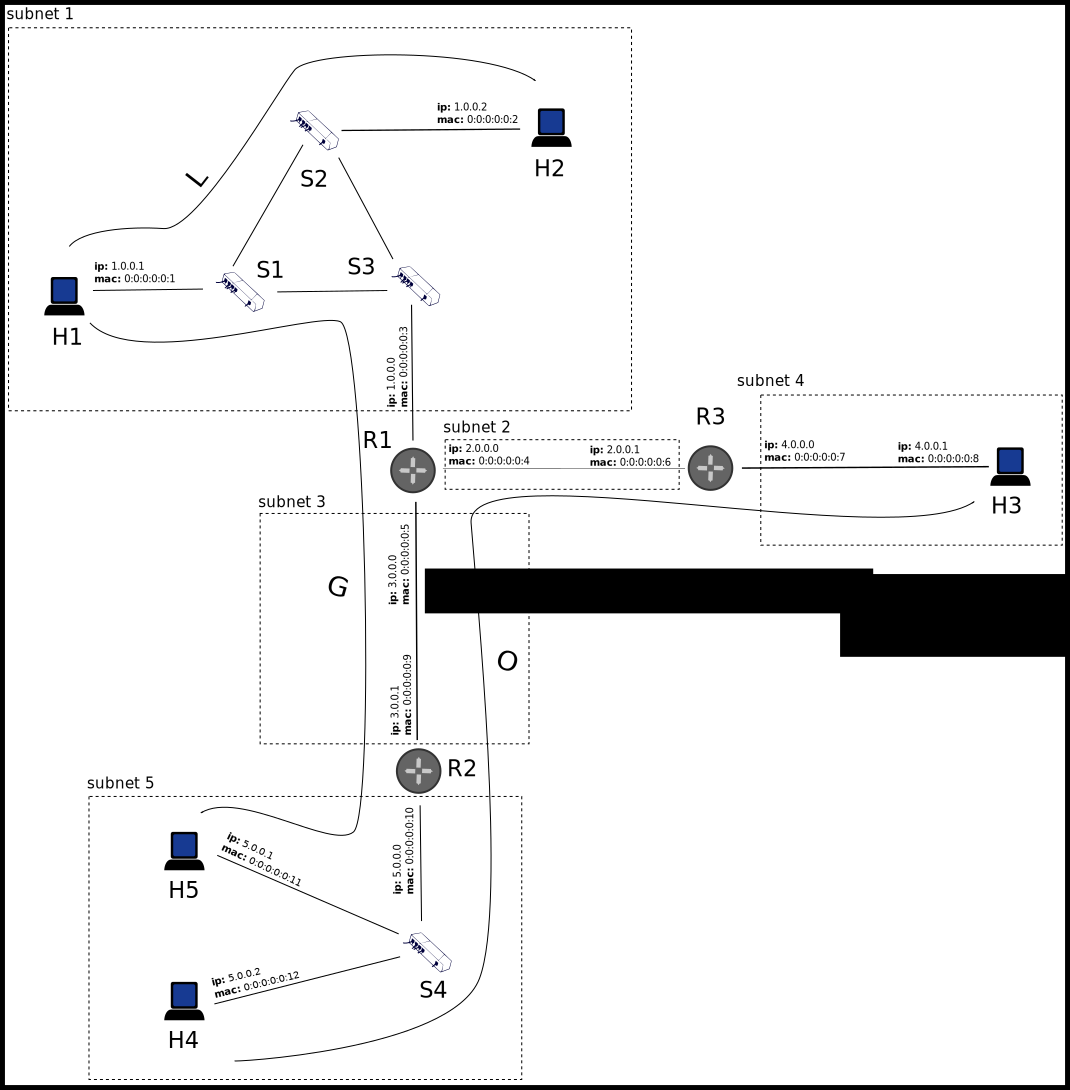
\includegraphics[width = 0.8\textwidth]{img/png/scenario.png}
    \caption{Escenario implementado.}
    \label{figure: case stady}
\end{figure}

Como ya fue mencionado, en este trabajo no se implementaron algoritmos dinamicos para completar las routing y forwarding tables, las mismas son completadas a mano. A continuación, se presentan tablas con las entradas seteadas para este escenario, las mismas están pensadas para el correcto funcionamiento de la red.

\begin{table}[!htb]
\rowcolors{1}{}{lightgray}
\centering
\begin{tabular}{c|c|c|c|c}
    \rowcolor[gray]{.1} \color{white}Network & \color{white}Netmask & \color{white}Nexthope & \color{white}Metric & \color{white}Description\\
    1.0.0.2 & 255.255.255.255 & 1.0.0.2 & 1 & Host 2 \\
    -&-&-&-&-\\
    -&-&-&-&-\\
\end{tabular}
\caption{Routing table del host 1.}
\label{tab:routing host 1}
\end{table}

\section{Resultados}
\section{Conclusiones}
\section{Trabajo futuro}
\section{References}
\bibliographystyle{plain}
\bibliography{references}

\end{document}